\documentclass[a4paper]{article}

%% Language and font encodings
\usepackage[english]{babel}
\usepackage[utf8x]{inputenc}
\usepackage[T1]{fontenc}

%% Sets page size and margins
\usepackage[a4paper,top=3cm,bottom=2cm,left=3cm,right=3cm,marginparwidth=1.75cm]{geometry}

%% Useful packages
\usepackage{amsmath}
\usepackage{graphicx}
\usepackage[colorinlistoftodos]{todonotes}
\usepackage[colorlinks=true, allcolors=blue]{hyperref}

\title{Homework 2: Solutions\\
600.482/682 Deep Learning\\
Fall 2018}
\author{Kaushik Srinivasan}

\begin{document}
\maketitle
With collaboration with Nathan Vallapureddy

\vspace{5mm}
\begin{enumerate}
	\item 
	\begin{gather*}
		f(x_1, x_2, w_1, w_2) = (1 + e^{-(w_1x_1-w_2x_2)})^{-1}\\
		f(-1, 1.5, 2, -2) = \frac{1}{(1 + e^{-1})}\\
		\frac{\partial f}{\partial w_1} = \frac{x_1}{(1 + e^{-(w_1x_1-w_2x_2)})^{2}} = \frac{-1}{(1+e^{-1})^2}\\
		\frac{\partial f}{\partial w_w} = \frac{-x_2}{(1 + e^{-(w_1x_1-w_2x_2)})^{2}} = \frac{-1.5}{(1+e^{-1})^2}\\
		\frac{\partial f}{\partial x_1} = \frac{w_1}{(1 + e^{-(w_1x_1-w_2x_2)})^{2}} = \frac{2}{(1+e^{-1})^2}\\
		\frac{\partial f}{\partial x_2} = \frac{-w_2}{(1 + e^{-(w_1x_1-w_2x_2)})^{2}} = \frac{2}{(1+e^{-1})^2}\\
	\end{gather*}
	\begin{center}
	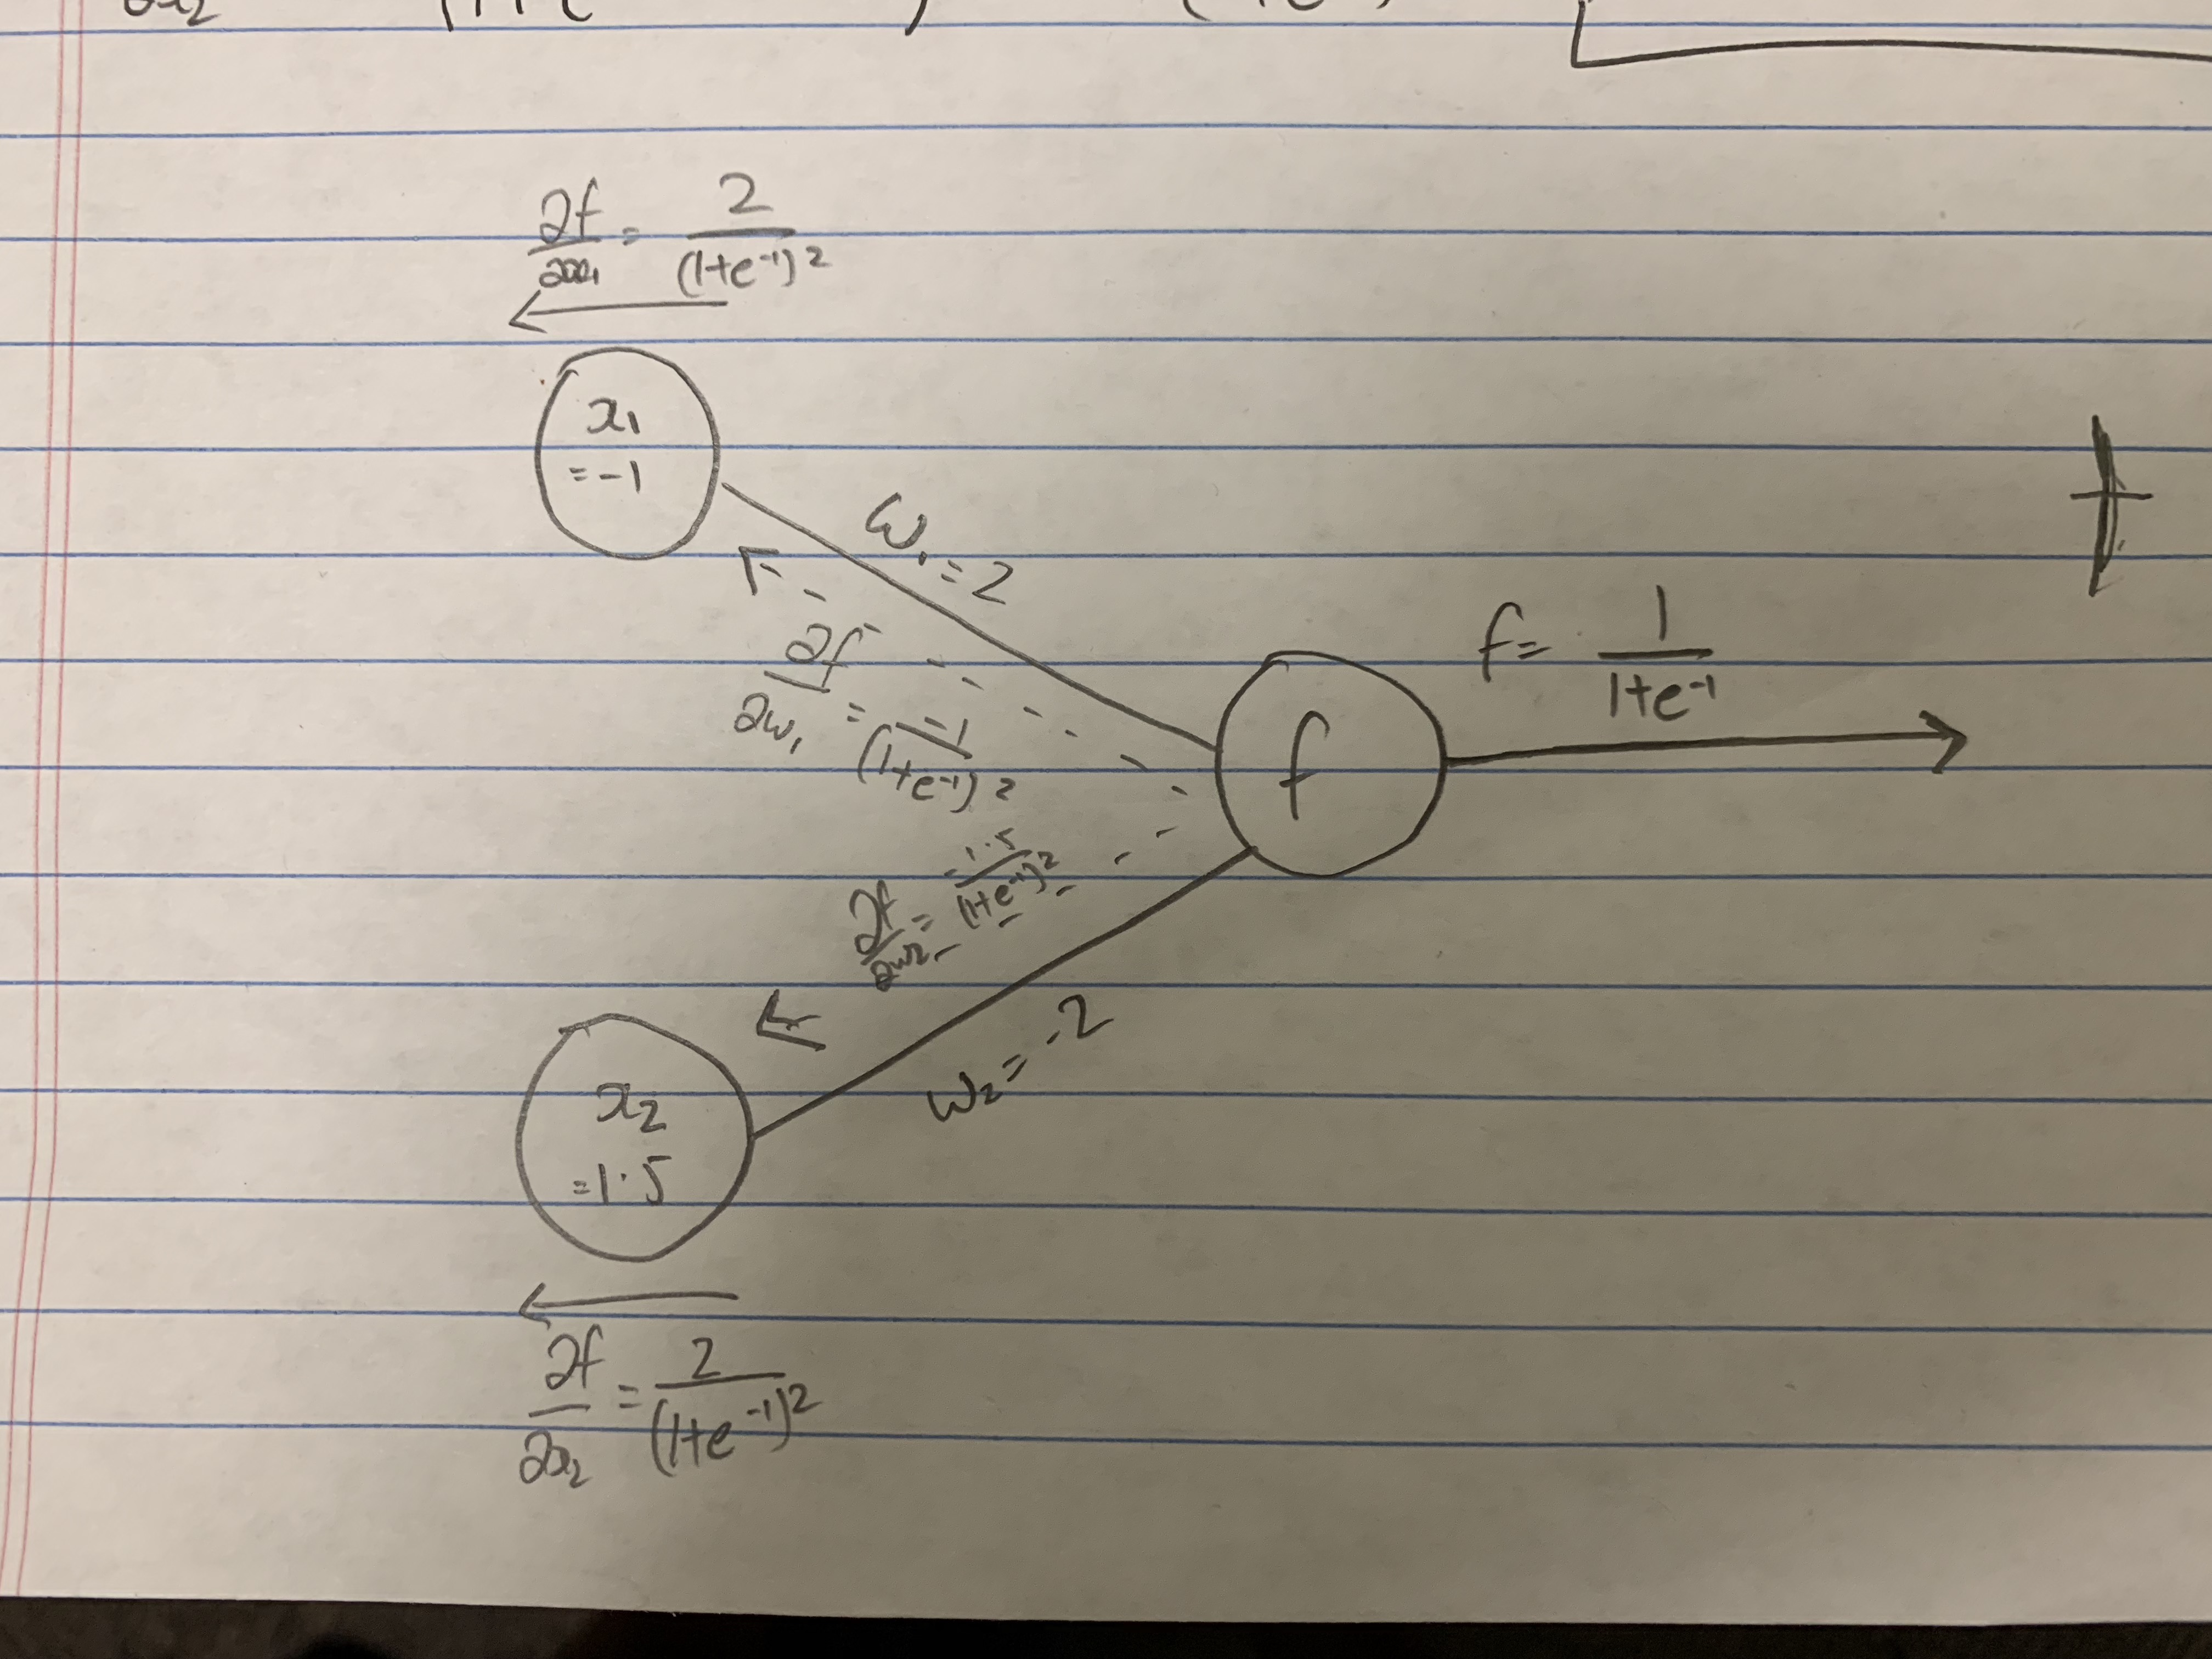
\includegraphics[scale=0.05]{IMG_0444}		
	\end{center}

	\item 
	\begin{enumerate}
	\item 
	\begin{align*}
		O(D, \theta) & = -\sum_i \log[z_i^{y_i} (1-z_i)^{(1-yi)}]\\
		& = -\sum_i y_i \log z_i + (1-y_i) \log (1-z_i)\\
		& = -\sum_i y_i \log \sigma(\theta^T x_i) + (1-y_i) \log (1-\sigma(\theta^T x_i))\\
		\nabla  O & = \bigg(\frac{\partial O}{\partial \theta_1}, \frac{\partial O}{\partial \theta_2}, \cdots, \frac{\partial O}{\partial \theta_n} \bigg)\\
		\frac{\partial O}{\partial \theta_j} & = \frac{\partial O}{\partial \theta_1} \bigg[ -\sum_i y_i \log \sigma(\theta^T x_i) + (1-y_i) \log (1-\sigma(\theta^T x_i)) \bigg]\\
		& = -\sum_i \bigg[ y_i \frac{\sigma ' (\theta^T x_i)}{\sigma(\theta^T x_i)} - (1-y_i) \frac{-\sigma ' (\theta^T x_i)}{1-\sigma(\theta^T x_i)} \bigg] \qquad \boxed{\sigma ' (\theta^T x_i) = \sigma(\theta^T x_i)\cdot(1 - \sigma (\theta^T x_i))}\\
		& = -\sum_i y_i (1 - \sigma (\theta^T x_i)) x_i^{(j)} - (1-y_i)\sigma (\theta^T x_i) x_i^{(j)}\\
	\end{align*}
	\begin{gather*}
		\boxed{\frac{\partial O}{\partial \theta_j} = -\sum_i (y_i - \sigma (\theta^T x_i)) x_i^{(j)}}\\
		\boxed{\frac{\partial^2 O}{\partial \theta_j \theta_k} = \sum_i \sigma (\theta^T x_i)\cdot (1-\sigma (\theta^T x_i)) x_i^{(j)} x_i^{(k)}}\\\\
		g + H \Delta \theta = 0 \Longrightarrow \boxed{\Delta \theta = H^{-1}g}
	\end{gather*}
	\item Check Code
	\item Code submitted
	\end{enumerate}
	\item 
	\begin{enumerate}
	\item 
	\begin{equation*}
		P(y = k | x, \theta) = \frac{exp\{ \theta_k^T x\}}{\sum_j exp\{\theta_j^T x\}}
	\end{equation*}
	\begin{align*}
		O(D; \theta) & = \prod_i \prod_k \bigg(\frac{exp\{ \theta_k^T x_i\}}{\sum_j exp\{\theta_j^T x_i\}} \bigg)^{I_{\{y_i = k\}}}\\
		-\log(O(D; \theta)) & = -log\bigg(\prod_i \prod_k \bigg(\frac{exp\{ \theta_k^T x_i\}}{\sum_j exp\{\theta_j^T x_i\}} \bigg)^{I_{\{y_i = k\}}} \bigg)\\
		& = -\bigg(  \sum_i \sum_k I_{\{y_i = k\}}\theta_k^T x_i - \log( \sum_j exp\{\theta_j^T x_i\} ) \bigg)
	\end{align*}
	\item 
	\begin{equation*}
		\nabla -\log(O(D;\theta))
	\end{equation*}
	\begin{align*}
		& = \sum_i \frac{\partial}{\partial \theta_k^{(n)}} (\theta_k^T x_i - \log (\sum_j \exp \{ \theta_j^T x_i) \} )\\
		& = \bigg( \sum_i \frac{\partial}{\partial \theta_k^{(n)}} \theta_k^T x_i \bigg) - \bigg( \sum_i \frac{\partial}{\partial \theta_k^{(n)}} \log\big( \sum_j exp\{ \theta_j^T x_i \} \big) \bigg)\\
		& = \sum_i x_i^{(n)} - \sum_i \frac{\frac{\partial}{\partial \theta_k^{(n)}} \sum_j exp \{\theta_j^T x_i \} }{\sum_j exp \{\theta_j^T x_i \}}\\
		& = \sum_i x_i^{(n)} - \sum_i \frac{  exp \{\theta_j^T x_i \} \frac{\partial}{\partial \theta_k^{(n)}} \theta_j^T x_i }{\sum_j exp \{\theta_j^T x_i \}}\\
		& = \sum_i x_i^{(n)} - \sum_i \frac{exp \{\theta_k^T x_i \} x_i^{(n)}}{\sum_j exp \{\theta_j^T x_i \}}\\
		& = \sum_i x_i^{(n)} \bigg( 1 - \frac{exp \{\theta_k^T x_i \}}{\sum_j exp \{\theta_j^T x_i \}} \bigg)
	\end{align*}
	\item check code
	\end{enumerate}
\end{enumerate}
\end{document}
